\documentclass[border=2pt]{standalone}
\usepackage{tikz}
\usetikzlibrary{arrows.meta,positioning,calc,fit,backgrounds,shapes.geometric}
\usepackage{amsmath,amssymb}
\usepackage{times}
\definecolor{ink}{HTML}{243447}
\definecolor{cA}{HTML}{4477AA}
\definecolor{cB}{HTML}{CC6677}
\definecolor{cAu}{HTML}{44AA99}
\definecolor{cS}{HTML}{CCAA33}
\definecolor{grn}{HTML}{228833}
\definecolor{rose}{HTML}{AA3377}
\definecolor{inst}{HTML}{F2E3B3}
\tikzset{
 pap/.style={circle,draw=ink,line width=.6pt,minimum size=15pt,inner sep=0pt,font=\scriptsize\bfseries,text=white},
 aut/.style={rectangle,draw=ink,line width=.6pt,minimum size=13pt,inner sep=0pt,fill=cAu,font=\scriptsize\bfseries,text=white},
 sub/.style={diamond,draw=ink,line width=.6pt,minimum size=17pt,inner sep=0pt,fill=cS,font=\scriptsize\bfseries,text=white},
 gone/.style={draw=ink!35,fill=ink!8,text=ink!40,dashed},
 ed/.style={draw=ink,line width=.7pt},
 msg/.style={-{Stealth[length=4pt]},line width=.9pt,draw=rose},
 ptitle/.style={font=\footnotesize\bfseries,text=ink,anchor=west},
 note/.style={font=\scriptsize,text=ink,align=center},
}

\tikzset{
 stage/.style={draw=ink!50,rounded corners=3pt,line width=.5pt,minimum width=2.78cm,minimum height=3.3cm,anchor=north west},
 stnum/.style={circle,fill=ink,text=white,font=\scriptsize\bfseries,inner sep=1.2pt},
 sname/.style={font=\scriptsize\bfseries,text=ink,anchor=west},
 small/.style={font=\fontsize{5.9}{6.8}\selectfont,text=ink,align=center},
 vec/.style={draw=ink,fill=#1,minimum width=4pt,minimum height=11pt,inner sep=0pt},
 flow/.style={-{Stealth[length=4pt]},line width=1pt,draw=ink!60},
}
\begin{document}
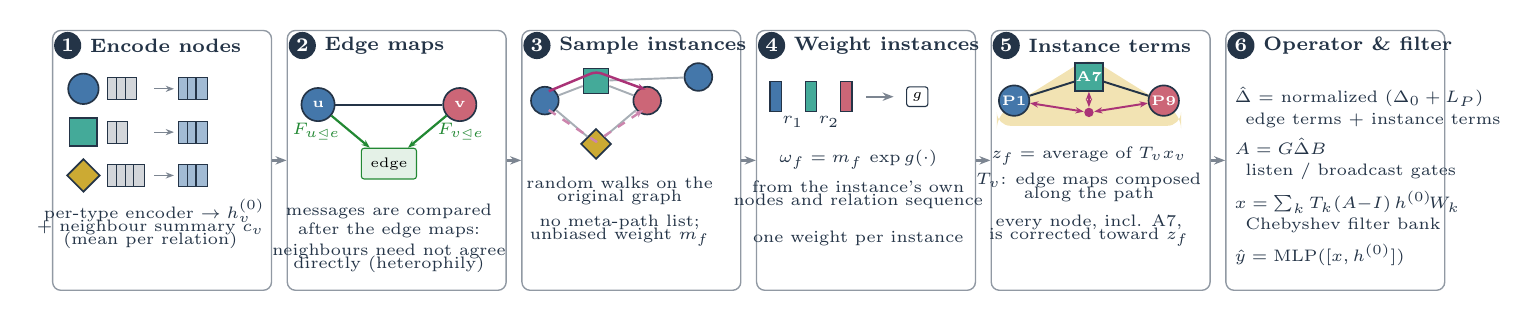
\begin{tikzpicture}
\def\W{2.98}
\foreach \i/\t in {0/Encode nodes,1/Edge maps,2/Sample instances,3/Weight instances,4/Instance terms,5/Operator \& filter}{
  \node[stage] (B\i) at (\i*\W,0) {};
  \node[stnum] at ($(B\i.north west)+(0.2,-0.2)$) {\the\numexpr\i+1\relax};
  \node[sname] at ($(B\i.north west)+(0.36,-0.2)$) {\t};
}
\foreach \i in {0,...,4}{ \pgfmathtruncatemacro\j{\i+1} \draw[flow] (B\i.east)--(B\j.west); }
% ---- 1 encode
\begin{scope}[shift={(0.25,-0.75)}]
 \node[pap,fill=cA,minimum size=11pt] (e1) at (0.15,0) {};
 \node[aut,minimum size=10pt] (e2) at (0.15,-0.55) {};
 \node[sub,minimum size=12pt] (e3) at (0.15,-1.1) {};
 \foreach \y/\w in {0/3,-0.55/2,-1.1/4}{\foreach \k in {1,...,\w}{\node[vec=ink!20,minimum height=8pt] at (0.42+\k*0.11,\y) {};}}
 \foreach \y in {0,-0.55,-1.1}{\draw[-{Stealth[length=3pt]},ink!60] (1.05,\y)--(1.3,\y);
   \foreach \k in {1,...,3}{\node[vec=cA!50,minimum height=8pt] at (1.32+\k*0.11,\y) {};}}
 \node[small] at (1.05,-1.55) {per-type encoder $\to h^{(0)}_v$};
 \node[small] at (1.0,-1.85) {+ neighbour summary $c_v$\\[-2pt](mean per relation)};
\end{scope}
% ---- 2 edge maps
\begin{scope}[shift={(\W+0.25,-0.95)}]
 \node[pap,fill=cA,minimum size=12pt] (u) at (0.15,0) {\tiny u};
 \node[pap,fill=cB,minimum size=12pt] (v) at (1.95,0) {\tiny v};
 \node[draw=grn,fill=grn!12,rounded corners=1pt,minimum width=0.5cm,minimum height=0.32cm,font=\tiny] (es) at (1.05,-0.75) {edge};
 \draw[ed] (u)--(v);
 \draw[-{Stealth[length=3pt]},grn,line width=.8pt] (u) -- node[small,left,text=grn]{$F_{u\trianglelefteq e}$} (es);
 \draw[-{Stealth[length=3pt]},grn,line width=.8pt] (v) -- node[small,right,text=grn]{$F_{v\trianglelefteq e}$} (es);
 \node[small] at (1.05,-1.35) {messages are compared};\node[small] at (1.05,-1.6) {after the edge maps:};
 \node[small] at (1.05,-1.95) {neighbours need not agree\\[-2pt]directly (heterophily)};
\end{scope}
% ---- 3 WISP
\begin{scope}[shift={(2*\W+0.3,-0.9)}]
 \node[pap,fill=cA,minimum size=10pt] (s1) at (0,0) {};
 \node[aut,minimum size=9pt] (s2) at (0.65,0.25) {};
 \node[pap,fill=cB,minimum size=10pt] (s3) at (1.3,0) {};
 \node[sub,minimum size=11pt] (s4) at (0.65,-0.55) {};
 \node[pap,fill=cA,minimum size=10pt] (s5) at (1.95,0.3) {};
 \draw[ed,ink!40] (s1)--(s2)--(s3) (s1)--(s4)--(s3) (s2)--(s5);
 \draw[-{Stealth[length=3pt]},rose,line width=.9pt,rounded corners=2pt] ($(s1)+(0.05,0.12)$)--($(s2)+(0,0.12)$)--($(s3)+(-0.02,0.14)$);
 \draw[-{Stealth[length=3pt]},rose!60,line width=.9pt,dashed] ($(s1)+(0.05,-0.12)$)--($(s4)+(0,0.03)$)--($(s3)+(-0.05,-0.12)$);
 \node[small] at (0.95,-1.15) {random walks on the\\[-2pt]original graph};
 \node[small] at (0.95,-1.65) {no meta-path list;\\[-2pt]unbiased weight $m_f$};
\end{scope}
% ---- 4 weight
\begin{scope}[shift={(3*\W+0.25,-0.85)}]
 \foreach \x/\c in {0/cA,0.45/cAu,0.9/cB}{\node[vec=\c] at (\x,0) {};}
 \node[small] at (0.22,-0.32) {$r_1$}; \node[small] at (0.68,-0.32) {$r_2$};
 \draw[flow,line width=.7pt] (1.15,0)--(1.5,0);
 \node[draw=ink,rounded corners=1pt,font=\tiny,inner sep=2pt] (g) at (1.8,0) {$g$};
 \node[small] at (1.05,-0.8) {$\omega_f = m_f\,\exp g(\cdot)$};
 \node[small] at (1.05,-1.25) {from the instance's own\\[-2pt]nodes and relation sequence};
 \node[small] at (1.05,-1.8) {one weight per instance};
\end{scope}
% ---- 5 instance term
\begin{scope}[shift={(4*\W+0.3,-0.9)}]
 \begin{scope}[on background layer]
 \fill[inst,rounded corners=5pt] (-0.22,-0.18)--(0.95,0.55)--(2.12,-0.18)--(2.12,-0.32)--(-0.22,-0.32)--cycle;\end{scope}
 \node[pap,fill=cA,minimum size=11pt] (i1) at (0,0) {\tiny P1};
 \node[aut,minimum size=10pt] (i2) at (0.95,0.3) {\tiny A7};
 \node[pap,fill=cB,minimum size=11pt] (i3) at (1.9,0) {\tiny P9};
 \draw[ed] (i1)--(i2)--(i3);
 \node[circle,fill=rose,inner sep=1.2pt] (zz) at (0.95,-0.15) {};
 \foreach \n in {i1,i2,i3}{\draw[msg,line width=.7pt,{Stealth[length=3pt]}-{Stealth[length=3pt]}] (zz)--(\n);}
 \node[small] at (0.95,-0.7) {$z_f=$ average of $T_v x_v$};
 \node[small] at (0.95,-1.1) {$T_v$: edge maps composed\\[-2pt]along the path};
 \node[small] at (0.95,-1.65) {every node, incl. A7,\\[-2pt]is corrected toward $z_f$};
\end{scope}
% ---- 6 operator
\begin{scope}[shift={(5*\W+0.02,-0.75)}]
 \node[small,align=left,anchor=north west] at (-0.02,0.15) {$\hat\Delta$ = normalized $(\Delta_0+L_P)$\\[1pt]
 \phantom{x}edge terms + instance terms\\[3pt]
 $A=G\hat\Delta B$\\[1pt] \phantom{x}listen / broadcast gates\\[3pt]
 $x=\sum_k T_k(A{-}I)\,h^{(0)}\!W_k$\\[1pt] \phantom{x}Chebyshev filter bank\\[3pt]
 $\hat y=\mathrm{MLP}([x,h^{(0)}])$};
\end{scope}
\end{tikzpicture}
\end{document}
